\section{Planificación temporal}
\par Mediante Microsoft Project se ha realizado un diagrama de Gantt mostrando la planificación del proyecto de forma semanal. El proyecto tiene los siguientes hitos:
\begin{itemize}
	\item \textbf{Hito G1:} 
	\begin{itemize}
		\item Presentación de la empresa
		\item Vídeo de la empresa
	\end{itemize}
	\item \textbf{Hito G2:}
	\begin{itemize}
		\item Planificación temporal
	\end{itemize}
	\item \textbf{Hito P1:}
	\begin{itemize}
		\item Información general - Introducción
		\item Presupuesto
		\item Propuesta de contrato
		\item Organización y gestión del proyecto
		\item Estudio de Viabilidad
		\item Análisis de riesgos
		\item Plan de gestión de la calidad
		\item Plan de gestión de la configuración
		\item Casos de uso expandidos
		\item Casos de uso de alto nivel
		\item Modelo de datos
		\item Navegación
	\end{itemize}
	\item \textbf{Hito G3:}
	\begin{itemize}
		\item Estimación de tamaño y esfuerzo
		\item Casos de uso reales
		\item Diagrama de clases
		\item Modelos de datos específicos
		\item Interfaces de usuario
		\item Desarrollo
		\item Plan de pruebas
		\item Plan de implantación
	\end{itemize}
	\item \textbf{Hito G4: Auditoría}
	\item \textbf{Hito E2: Fin}
	\begin{itemize}
		\item Instalación del sistema
	\end{itemize}
\end{itemize}

\par A continuación se incluye la captura de MS Project:
\begin{figure}
  \centering
    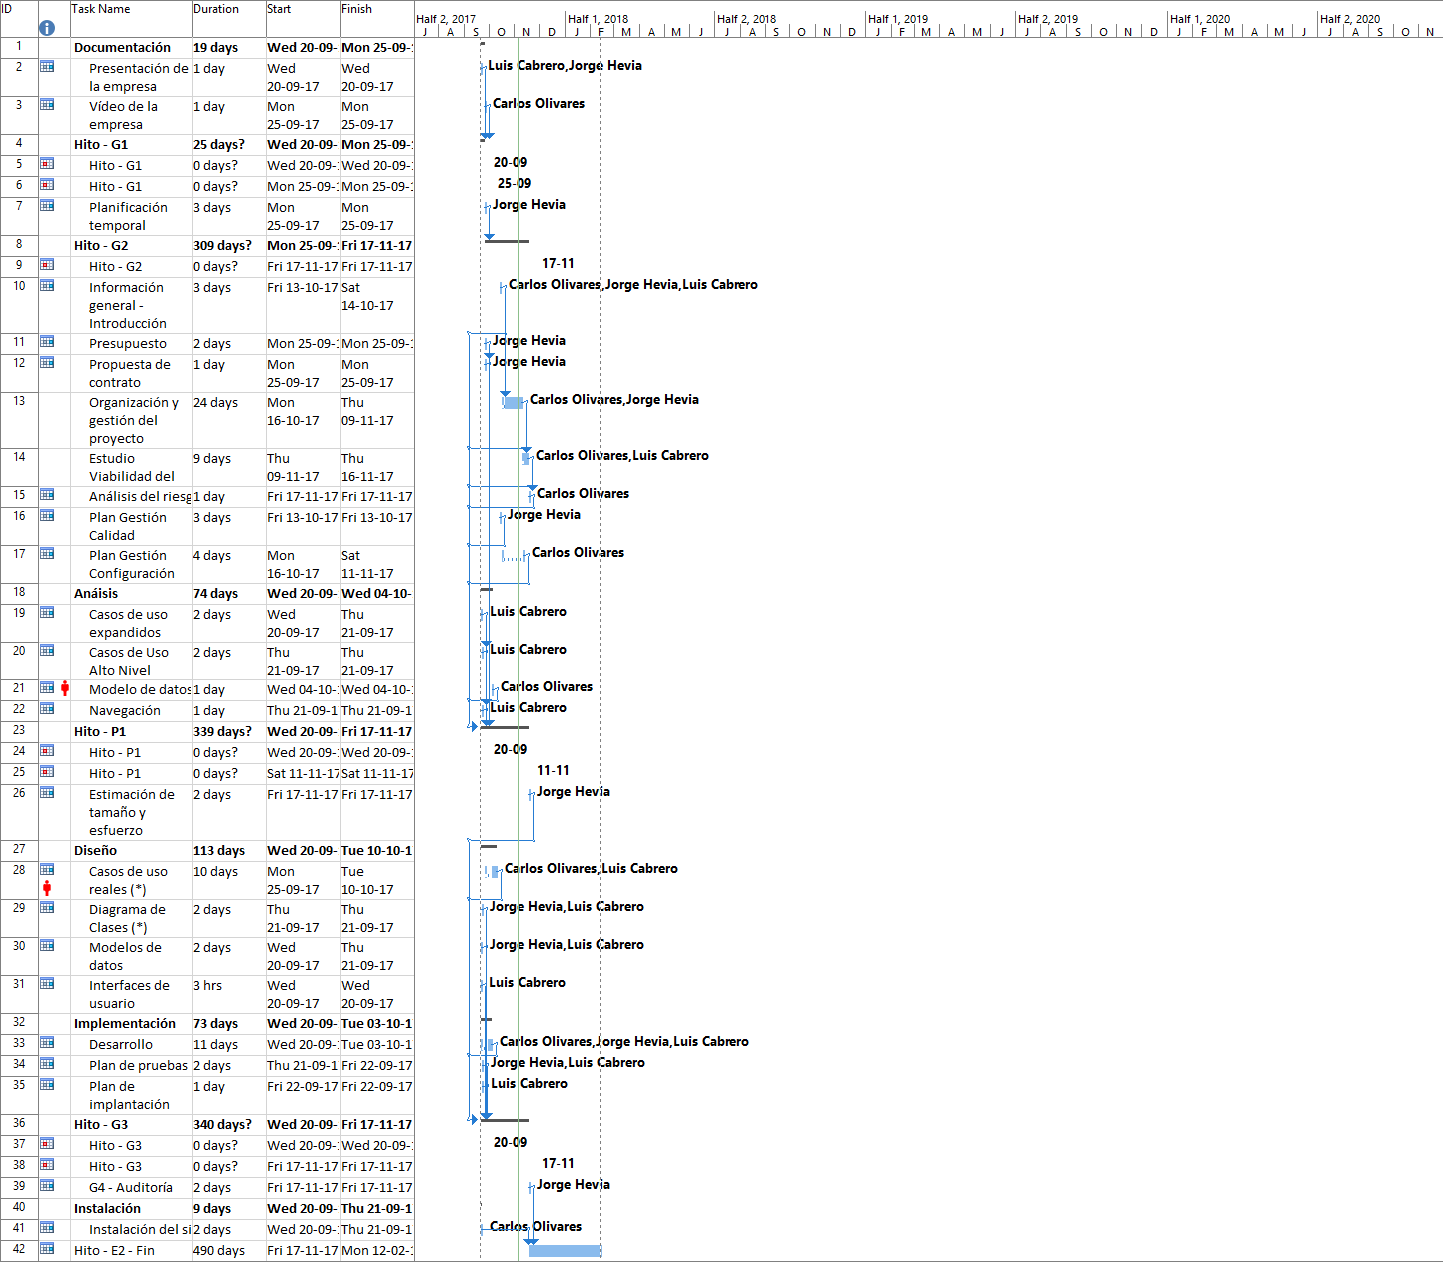
\includegraphics[width=0.8\textwidth]{img/gantt.png}
  \caption{Captura de diagrama de Gantt en MS Project}
  \label{fig:gantt}
\end{figure}
Figure \ref{fig:gantt} Diagrama de Gantt.